\documentclass[main.tex]{subfiles}
\begin{document}
\begin{enumerate}

\subsection{Section 6}

\item Provide clear explanations to the following questions:

    \begin{enumerate}
        \item Using band-theory and energy-related arguments, explain why a metal conducts, an insulator blocks current, and a semiconductor conducts current only under certain situations.
        \item A PN junction is used as a photodetector. Assume that light is shining on all parts of the diode equally. Which part of the photodiode is most critical for photo detection and why? In this application, should the devices be under forward or reverse bias?
        \item After repeated operations of a PMOS MOSFET, hole-type interface traps are formed in the Si-SiO2 interface, does this process increase or decrease the threshold voltage? Draw the band-diagram and the sub-threshold IV curve to illustrate your answer.
    \end{enumerate}

\item MOS Capacitor

    \begin{enumerate}
        \item Draw the band diagram of a MOS system where the "metal" work function $\Phi_{\mathrm{M}}$ is larger than the silicon work function $\Phi_{\mathrm{S}}$. Assume that there are no applied voltages at the p-type substrate (doping $\mathrm{N}_{\mathrm{A}}$) and the gate. On the diagram clearly label the following parameters and functions: electron affinity in the semiconductor $\chi_{\mathrm{Sc}}$, the Fermi level $\mathrm{E}_{\mathrm{F}}$, the conduction and valance band edges $\mathrm{E}_{\mathrm{c}}$ and $\mathrm{E}_{\mathrm{V}}$, the band-gap $\mathrm{E}_{\mathrm{g}}$, the mid-gap $\mathrm{E}_{i}$, the thickness of the oxide $\mathrm{t}_{\mathrm{ox}}$, the potential drop in the oxide $\phi_{\mathrm{ox}}$, and the potential drop in the semiconductor $\phi(\mathrm{x})$
        \item For this device, what is the most likely outcome when no voltages are applied: inversion or accumulation? Why?
        \item Poly-Silicon Gate Depletion (refer to Figure \ref{fig:17q_a}): Assume the voltage $\mathrm{V}_{\mathrm{ox}} = \qty{1}{\volt}$ across a $\qty{2}{\nano\meter}$ thin \ch{SiO2} oxide. The $\mathrm{P}^{+}$ poly gate doping is $\mathrm{N}_{\text {poly }}=1 \times 10^{19} \mathrm{~cm}^{-3}$ and the substrate is n-doped with $\mathrm{N}_{\mathrm{D}}=10^{17} \mathrm{~cm}^{-3}$. Find the poly depletion width, $\mathrm{W}_{\mathrm{dep }}$.
    \end{enumerate}
    
\begin{figure}
\centering\fbox{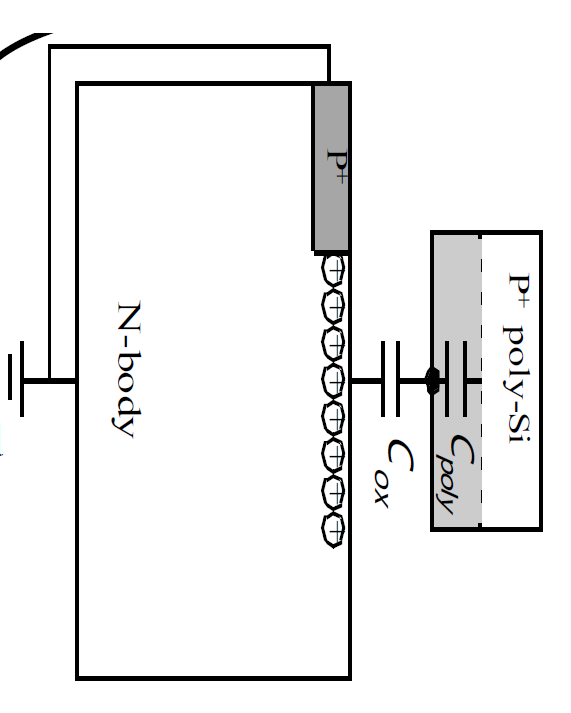
\includegraphics[width=3.0in]{figures/2018s/17q_a.png}}
\caption{Schematic of the poly depletion capacitances upon gating this MOS capacitor. $\mathrm{T}=300\mathrm{K}$}. Gate and body are Silicon. The gate ocide is \ch{SiO2}, $\mathrm{t}_{\mathrm{ox}} = 2 \mathrm{~nm}$}
\label{fig:17q_a}
\end{figure}

\item Basic \textit{pn}-junction operation.\\

Consider the ideal so-called "long-base" abrupt \textit{pn}-junction silicon diode that has a uniform cross section and constant doping on both sides of the \textit{pn}-junction. The diode is doped as follows: $\mathrm{N}_{\mathrm{a}}=8.0 \times 10^{16} \mathrm{~cm}^{-3}$ \textit{p}-type and $\mathrm{N}_{\mathrm{d}}=1 \mathrm{x} 10^{16} \mathrm{~cm}^{-3}$ \textit{n}-type. For this material, the minority-carrier lifetimes are: $\tau_{\mathrm{n}}=4 \times 10^{-6} \mathrm{~s}$ and $\tau_{\mathrm{p}}=1 \times 10^{-6} \mathrm{~s}$, respectively. You may assume that the effects within the space-charge region are negligible and that the minority carriers flow only by diffusion in the charge neutral regions.

    \begin{enumerate}
        \item Draw/sketch the band-diagram for this system. Also, plot the electrostatic potential, the net charge density and the and the corresponding electric field.
        \item Determine the value of the built-in potential across the \textit{pn}-junction.
        \item Calculate the density of the minority carriers at the edge of the space-charge region for a forward bias of 0.3V.
        \item Under bias condition, calculate and plot the minority and majority carrier currents as a function of distance from the junction.
    \end{enumerate}

\end{enumerate}
\end{document}